\section{مروری بر کارهای مرتبط} % Corresponds to 1.5
\label{sec:related-work}

\subsection{رادارهای پزشکی و کاربردهای آن‌ها} % Corresponds to 1.5.1
\label{sec:medical-radars}

در سال‌های اخیر، فناوری رادار به‌ویژه در کاربردهای پزشکی مورد توجه ویژه‌ای قرار گرفته است.\cite{li2013review} برخلاف کاربردهای سنتی رادار در صنایع نظامی و خودرو، امروزه رادارها در زمینه‌هایی مانند پایش علائم حیاتی (ضربان قلب و نرخ تنفس)، تشخیص سقوط بیماران، شناسایی حرکت‌های غیرارادی بدن، و پایش بیماران در اتاق مراقبت‌های ویژه مورد استفاده قرار می‌گیرند. این سیستم‌ها، برای بیماران با شرایط خاص، نوزادان و سالمندان مزیت چشم‌گیری دارند.
برخی پژوهش‌ها به بررسی عملکرد رادارهای میلی‌متری برای شناسایی علائم حیاتی در اتاق‌های بیمارستانی یا حتی در محیط خانگی پرداخته‌اند. برای مثال، از رادارهای \lr{Doppler} برای اندازه‌گیری نرخ تنفس استفاده شده و مشخص شده که این رادارها قادر به تشخیص تغییرات کوچک در قفسه سینه فرد هستند. همچنین رادارهای \lr{FMCW} و \lr{UWB} در این زمینه در حال رشد چشمگیری‌اند، چرا که قابلیت تفکیک مکانی و حساسیت بالاتری دارند.

\subsection{اندازه‌گیری ضربان قلب با رادار: روش‌های \lr{CW}، \lr{FMCW}، و \lr{UWB}} % Corresponds to 1.5.2
\label{sec:heart-rate-radar-methods}

اندازه‌گیری ضربان قلب با رادار، با استفاده از روش‌های مختلفی امکان‌پذیر است که هرکدام مزایا و محدودیت‌های خاص خود را دارند:
\begin{itemize}
    \item \textbf{رادار موج پیوسته (\lr{CW})}: در این روش، رادار سیگنال سینوسی با فرکانس ثابت ارسال می‌کند و تغییرات فاز سیگنال بازتاب‌شده را برای تشخیص حرکت‌های ظریف بدن (مثل ضربان قلب) تحلیل می‌کند. این روش ساده است، اما توان تفکیک مکانی ندارد و در محیط‌های با چند هدف یا نویز بالا عملکرد خوبی ندارد.
    \item \textbf{رادار \lr{FMCW (Frequency Modulated Continuous Wave)}}: این روش با استفاده از مدولاسیون خطی فرکانس، امکان تخمین فاصله و همچنین استخراج اطلاعات حرکت ظریف را فراهم می‌آورد. رادارهای \lr{FMCW} با دقت بالا می‌توانند ضربان قلب را در فاصله‌های مختلف و بدون تماس ثبت کنند. پژوهش‌هایی مانند \lr{Li et al. (2018)} و \lr{Wang et al. (2020)} به نتایج موفقی در این زمینه دست یافته‌اند و قابلیت استفاده از \lr{FMCW} را در شرایط متحرک یا پرنویز اثبات کرده‌اند.\cite{yue2020non}
    \item \textbf{رادار باند فوق‌گسترده (\lr{UWB})}: این نوع رادار با ارسال پالس‌های کوتاه و پهن‌باند، قادر به اندازه‌گیری دقیق موقعیت و حرکت است. مزیت آن توانایی بالا در تفکیک مکانی و کاهش اثرات تداخل می‌باشد. در عین حال، به دلیل الزامات تنظیمی و پیچیدگی سخت‌افزار، کاربرد آن در عمل ممکن است محدود شود.
\end{itemize}

\subsection{خلأها و چالش‌های موجود} % Corresponds to 1.5.3
\label{sec:gaps-challenges}

با وجود پیشرفت‌های قابل‌توجه در اندازه‌گیری ضربان قلب با استفاده از رادار، همچنان چالش‌ها و خلأهایی در این حوزه باقی مانده است:
\begin{enumerate}
    \item \textbf{نویز و تداخل حرکتی}: یکی از چالش‌های اصلی، تداخل ناشی از حرکت‌های بزرگ بدن یا حضور اشیاء متحرک در محیط است که می‌تواند بر روی سیگنال ضربان قلب اثر بگذارد و دقت اندازه‌گیری را کاهش دهد.
    \item \textbf{تفکیک ضربان قلب از نرخ تنفس}: در بسیاری از موارد، سیگنال‌های ناشی از تنفس قوی‌تر از سیگنال ضربان قلب هستند و استخراج دقیق ضربان قلب نیازمند فیلترینگ دقیق یا استفاده از الگوریتم‌های پردازش سیگنال پیشرفته است.\cite{adib2015smart}
    \item \textbf{نبود مدل استاندارد برای مقایسه عملکرد}: بیشتر تحقیقات از روش‌های خاص خود برای اندازه‌گیری و ارزیابی استفاده کرده‌اند و فقدان یک استاندارد یا دیتاست عمومی باعث دشواری در مقایسه دقیق میان روش‌ها می‌شود.
    \item \textbf{پیاده‌سازی در شرایط واقعی}: بسیاری از مطالعات در محیط‌های کنترل‌شده آزمایشگاهی انجام شده‌اند. پیاده‌سازی موفق در محیط‌های واقعی (مانند اتاق بیمار، خودرو یا منزل) نیازمند بهینه‌سازی طراحی آنتن، مدارات پردازش و حذف نویز محیطی است.
    \item \textbf{نیاز به الگوریتم‌های هوشمند پردازش سیگنال}: برای استخراج دقیق ضربان قلب از داده‌های راداری، به‌ویژه در حضور نویز و حرکات اضافی، نیاز به الگوریتم‌های پیشرفته یادگیری ماشین، پردازش سیگنال تطبیقی و تحلیل چند متغیره احساس می‌شود.
\end{enumerate}



\vspace{2cm}
\begin{center}
\begin{figure}[!h]
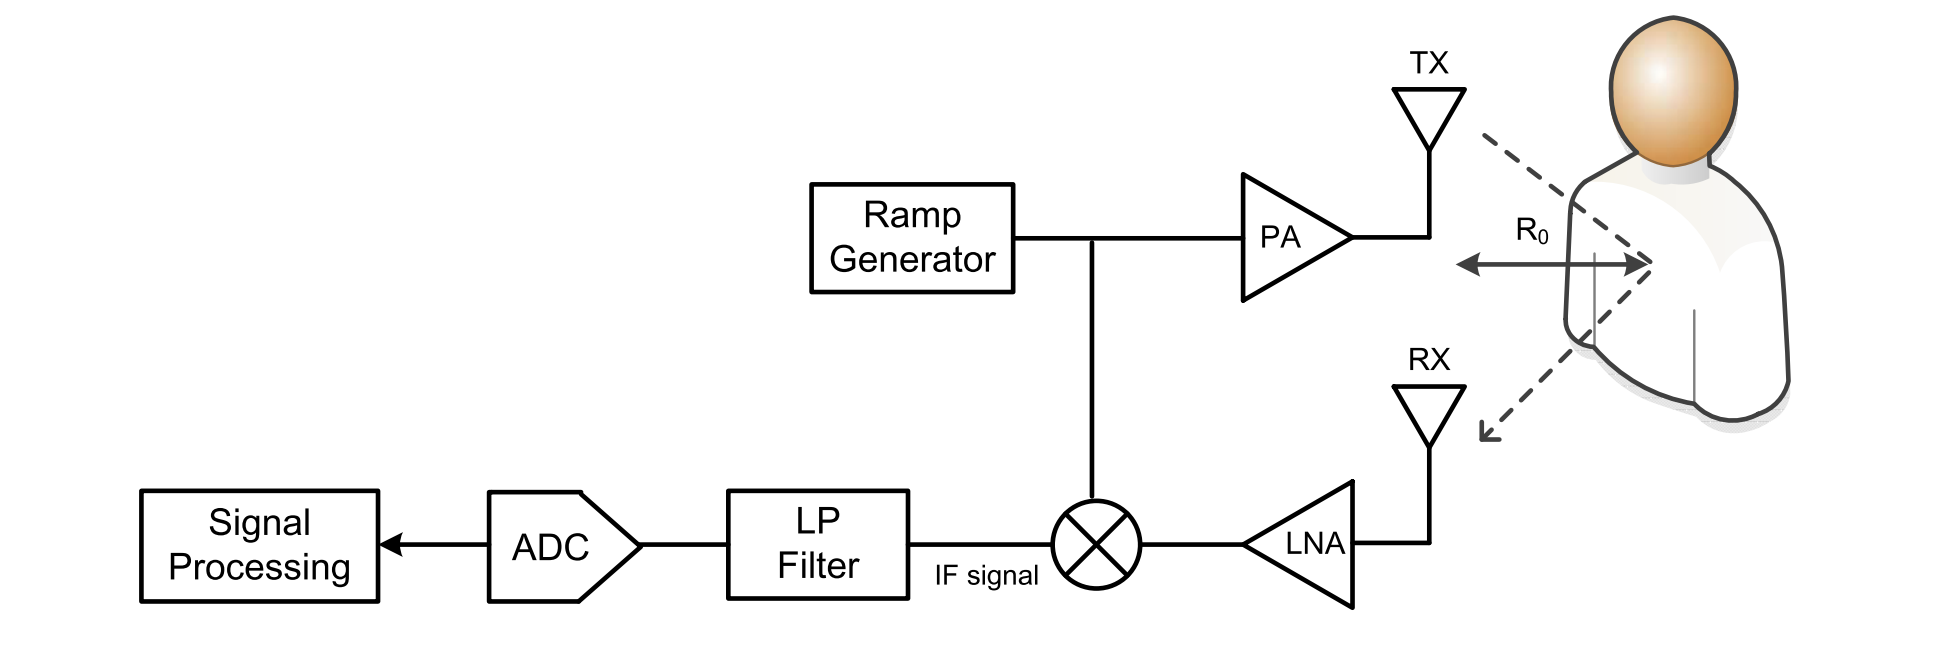
\includegraphics[height=4cm,width=12cm]{Images/chapter1/1-2.png}
\caption{بلاک دیاگرام رادار \lr{fmcw}.\cite{adib2015smart}
}
\end{figure}
\end{center}
\vspace{2cm}

